% Preamble -------------------------------------------------
\documentclass{beamer}\usepackage[]{graphicx}\usepackage[]{color}
%% maxwidth is the original width if it is less than linewidth
%% otherwise use linewidth (to make sure the graphics do not exceed the margin)
\makeatletter
\def\maxwidth{ %
  \ifdim\Gin@nat@width>\linewidth
    \linewidth
  \else
    \Gin@nat@width
  \fi
}
\makeatother

\definecolor{fgcolor}{rgb}{0.345, 0.345, 0.345}
\newcommand{\hlnum}[1]{\textcolor[rgb]{0.686,0.059,0.569}{#1}}%
\newcommand{\hlstr}[1]{\textcolor[rgb]{0.192,0.494,0.8}{#1}}%
\newcommand{\hlcom}[1]{\textcolor[rgb]{0.678,0.584,0.686}{\textit{#1}}}%
\newcommand{\hlopt}[1]{\textcolor[rgb]{0,0,0}{#1}}%
\newcommand{\hlstd}[1]{\textcolor[rgb]{0.345,0.345,0.345}{#1}}%
\newcommand{\hlkwa}[1]{\textcolor[rgb]{0.161,0.373,0.58}{\textbf{#1}}}%
\newcommand{\hlkwb}[1]{\textcolor[rgb]{0.69,0.353,0.396}{#1}}%
\newcommand{\hlkwc}[1]{\textcolor[rgb]{0.333,0.667,0.333}{#1}}%
\newcommand{\hlkwd}[1]{\textcolor[rgb]{0.737,0.353,0.396}{\textbf{#1}}}%
\let\hlipl\hlkwb

\usepackage{framed}
\makeatletter
\newenvironment{kframe}{%
 \def\at@end@of@kframe{}%
 \ifinner\ifhmode%
  \def\at@end@of@kframe{\end{minipage}}%
  \begin{minipage}{\columnwidth}%
 \fi\fi%
 \def\FrameCommand##1{\hskip\@totalleftmargin \hskip-\fboxsep
 \colorbox{shadecolor}{##1}\hskip-\fboxsep
     % There is no \\@totalrightmargin, so:
     \hskip-\linewidth \hskip-\@totalleftmargin \hskip\columnwidth}%
 \MakeFramed {\advance\hsize-\width
   \@totalleftmargin\z@ \linewidth\hsize
   \@setminipage}}%
 {\par\unskip\endMakeFramed%
 \at@end@of@kframe}
\makeatother

\definecolor{shadecolor}{rgb}{.97, .97, .97}
\definecolor{messagecolor}{rgb}{0, 0, 0}
\definecolor{warningcolor}{rgb}{1, 0, 1}
\definecolor{errorcolor}{rgb}{1, 0, 0}
\newenvironment{knitrout}{}{} % an empty environment to be redefined in TeX

\usepackage{alltt}
\usepackage[utf8]{inputenc}
\usepackage[ngerman]{babel}
\usepackage{adjustbox}
\usepackage{tikz}
  \usetikzlibrary{positioning, calc, decorations.pathreplacing, backgrounds, fit}
\usepackage{multirow}
\usepackage{graphicx}
\usepackage{caption}
\usepackage{booktabs}

\definecolor{grey538}{rgb}{240,240,240}

% Slides setup ---------------------------------------------
\usetheme{Berlin}
\usecolortheme{seagull}
\usefonttheme{professionalfonts}

\title{Zusammenfassung vom 5. Januar 2018}
\author{Dag Tanneberg\thanks{%
  \href{mailto:dag.tanneberg@uni-potsdam.de}%
    {dag.tanneberg@uni-potsdam.de}
  }
}
\institute[Universität Potsdam]{
  {\glqq}Forschungsdesign in den Sozialwissenschaften{\grqq}\\
  Universität Potsdam\\
  Lehrstuhl für Vergleichende Politikwissenschaft\\
  Wintersemester 2017/2018
}
\date{15. Januar 2018}
\IfFileExists{upquote.sty}{\usepackage{upquote}}{}
\begin{document}
\maketitle



\begin{frame}
\frametitle{Leitfragen der Sitzung}
  \begin{enumerate}
    \item Welche Fallstricke stellen sich einem Forschungsdesign?
    \item Was sind unsystematische bzw. systematische Messfehler?
    \item Wie wirken sich Messfehler aus?
    \item Wie gehe ich mit Messfehlern um??
  \end{enumerate}
\end{frame}

\begin{frame}
\frametitle{Welche Fallstricke stellen sich einem Forschungsdesign?}
  \textbf{Sehr viele!} Messfehler, Drittvariablen, Endogenität\dots
  \vfill
  \textbf{Wie wirken sich diese Fallstricke aus?}
  \begin{enumerate}
    \item \textbf{Effizienz}
    \begin{itemize}
      \item Wie stabil sind Ergebnisse bei wiederholter Analyse?
      \item [$\rightarrow$] Präzision eines Inferenzschlusses
    \end{itemize}
    \item \textbf{Bias}
    \begin{itemize}
      \item Werden Ergebnisse systematisch verfälscht?
      \item [$\rightarrow$] Erwartungstreue eines Inferenzschlusses
    \end{itemize}
  \end{enumerate}
\end{frame}

\begin{frame}
  \frametitle{Was sind unsystematische bzw. systematische Messfehler?}
  \begin{itemize}
    \item \textbf{Messen}
    \begin{itemize}
      \item regelgeleitete Zuordnung von Zahlen zu Objekten
      \item strukturtreue Abbildung der Realität
    \end{itemize}
    \item \textbf{Messfehler}
    \begin{itemize}
      \item Abweichung des Messergebnisses $x$ vom ``wahren'' Wert $\theta$
      \item unsystematische ($\epsilon$) oder systematische Abweichung ($u$)
    \end{itemize}
  \end{itemize}
  \begin{columns}
  \begin{column}{.3\textwidth}
      \begin{figure}
        \begin{tikzpicture}[
          grow = right, edge from parent/.style={draw,-latex},
          level distance = 8em, sibling distance = 8em, minimum size = 2em, inner sep = 0,
          scale = 1,
          background rectangle/.style = {fill = gray!10},%
          show background rectangle
        ]
          \tikzstyle {latent} = [draw, shape = circle, fill = white]
          \tikzstyle {observed} = [draw, shape = rectangle, fill = white]
          % place nodes
          \path node (0) [latent] at (-1,0) {$\theta$};
          \path node (1) [observed] at (0,0) {$x$};
          \path node (2) [latent] at (1,.6) {$\epsilon$};
          \path node (3) [latent] at (1,-.6) {$u$};
          % place edges
          \foreach \x in {0, 2, 3}
            { \draw [-latex] (\x) -- (1) ; } ;
          \begin{scope}[on background layer]
            \node [fill=grey538, fit = (0) (1) (2)] {};
          \end{scope}
        \end{tikzpicture}
      \end{figure}
    \end{column}
    \begin{column}{.7\textwidth}
      \begin{tabular}{*{3}{l}}
        ~ & \textbf{unsystematisch} & \textbf{systematisch}\\
        Abweichung & zufällig & immer gleich \\
        Beispiel & Erinnerungsfehler & Lügen \\
      \end{tabular}
    \end{column}
  \end{columns}
\end{frame}

\begin{frame}
\frametitle{Wie wirken sich Messfehler aus?}
\textbf{Es kommt darauf an.}
\begin{enumerate}
  \item Geht es um Beschreibung oder kausale Inferenz?
  \item Betrifft der Fehler die abhängige oder die unabh. Variable?
\end{enumerate}
\vfill

\begin{tabular}{l*{4}{c}}
\toprule
~ & \multicolumn{2}{c}{\textbf{Abhängige Variable}} & \multicolumn{2}{c}{\textbf{Unabh. Variable}}\\
~ & Deskription & Kausalität & Deskription & Kausalität\\ \midrule
unsystem. & Ineffizienz & Ineffizienz & Ineffizienz & Bias \\
systemat. & Bias & unerheblich$^*$ & Bias & unerheblich$^*$\\
\bottomrule
\multicolumn{5}{l}{$^*$ Gilt nur, wenn der Fehler \textit{alle} Untersuchungseinheiten betrifft.}
\end{tabular}
\end{frame}

\begin{frame}
  \frametitle{Effekt unsystematischer Messfehler auf kausale Inferenz}
\begin{knitrout}
\definecolor{shadecolor}{rgb}{0.969, 0.969, 0.969}\color{fgcolor}
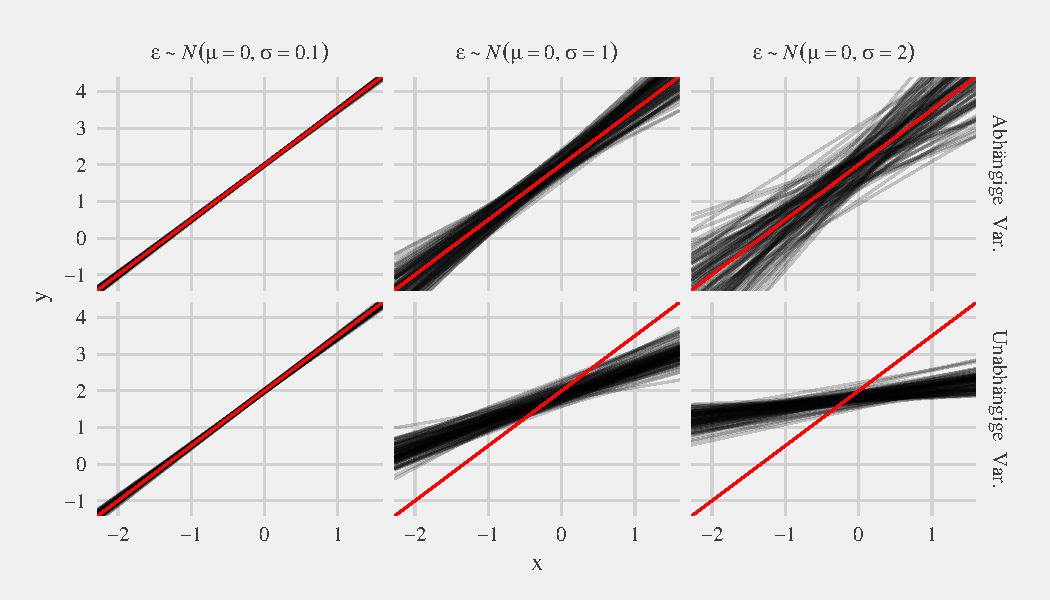
\includegraphics[width=\maxwidth]{figure/execute-error-simulation-1} 

\end{knitrout}
\end{frame}

\begin{frame}
  \frametitle{Wie gehe ich mit Messfehlern um?}
  \begin{enumerate}
    \item Konzept und Messung eng vermitteln
    \item multiple Indikatoren verwenden
    \item [$\rightarrow$] Merkmal mehrfach in unterschiedlicher Form erheben
    \item empirische Implikationen steigern
    \item [$\rightarrow$] Wie sollte sich die Beziehung $X \implies Y$ noch äußern?
    \item Effekt antizipieren und offen diskutieren
    \item [$\rightarrow$] Wird der Zusammenhang unter- oder überschätzt?
  \end{enumerate}
\end{frame}
\end{document}
